 \documentclass[a4paper]{article}
\usepackage{vntex}
%\usepackage[english,vietnam]{babel}
%\usepackage[utf8]{inputenc}

%\usepackage[utf8]{inputenc}
%\usepackage[francais]{babel}
\usepackage{a4wide,amssymb,epsfig,latexsym,multicol,array,hhline,fancyhdr}
\usepackage{booktabs}
\usepackage{amsmath}
\usepackage{lastpage}
\usepackage[lined,boxed,commentsnumbered]{algorithm2e}
\usepackage{enumerate}
\usepackage{color}
\usepackage{graphicx}							% Standard graphics package
\usepackage{array}
\usepackage{tabularx, caption}
\usepackage{multirow}
\usepackage[framemethod=tikz]{mdframed}% For highlighting paragraph backgrounds
\usepackage{multicol}
\usepackage{rotating}
\usepackage{graphics}
\usepackage{geometry}
\usepackage{setspace}
\usepackage{epsfig}
\usepackage{tikz}
\usepackage{listings}
\usepackage{xcolor}
\usetikzlibrary{arrows,snakes,backgrounds}
\usepackage{hyperref}
\hypersetup{urlcolor=blue,linkcolor=black,citecolor=black,colorlinks=true} 
%\usepackage{pstcol} 								% PSTricks with the standard color package

\newtheorem{theorem}{{\bf Định lý}}
\newtheorem{property}{{\bf Tính chất}}
\newtheorem{proposition}{{\bf Mệnh đề}}
\newtheorem{corollary}[proposition]{{\bf Hệ quả}}
\newtheorem{lemma}[proposition]{{\bf Bổ đề}}

\everymath{\color{blue}}
%\usepackage{fancyhdr}
\setlength{\headheight}{40pt}
\pagestyle{fancy}
\fancyhead{} % clear all header fields
\fancyhead[L]{
 \begin{tabular}{rl}
    \begin{picture}(25,15)(0,0)
    \put(0,-8){
\includegraphics[width=8mm, height=8mm]{logoITSGUsmall.png}}
    %\put(0,-8){\epsfig{width=10mm,figure=hcmut.eps}}
   \end{picture}&
	%\includegraphics[width=8mm, height=8mm]{hcmut.png} & %
	\begin{tabular}{l}
		\textbf{\bf \ttfamily Trường Đại học Sài Gòn}\\
		\textbf{\bf \ttfamily Khoa Công Nghệ Thông Tin}
	\end{tabular} 	
 \end{tabular}
}
\fancyhead[R]{
	\begin{tabular}{l}
		\tiny \bf \\
		\tiny \bf 
	\end{tabular}  }
\fancyfoot{} % clear all footer fields
\fancyfoot[L]{\scriptsize \ttfamily Bài tập lớn môn Phát triển phần mềm mã nguồn mở - Niên khóa 2023-2024}
\fancyfoot[R]{\scriptsize \ttfamily Trang {\thepage}/\pageref{LastPage}}
\renewcommand{\headrulewidth}{0.3pt}
\renewcommand{\footrulewidth}{0.3pt}


%%%
\setcounter{secnumdepth}{4}
\setcounter{tocdepth}{3}
\makeatletter
\newcounter {subsubsubsection}[subsubsection]
\renewcommand\thesubsubsubsection{\thesubsubsection .\@alph\c@subsubsubsection}
\newcommand\subsubsubsection{\@startsection{subsubsubsection}{4}{\z@}%
                                     {-3.25ex\@plus -1ex \@minus -.2ex}%
                                     {1.5ex \@plus .2ex}%
                                     {\normalfont\normalsize\bfseries}}
\newcommand*\l@subsubsubsection{\@dottedtocline{3}{10.0em}{4.1em}}
\newcommand*{\subsubsubsectionmark}[1]{}
\makeatother

\definecolor{dkgreen}{rgb}{0,0.6,0}
\definecolor{gray}{rgb}{0.5,0.5,0.5}
\definecolor{mauve}{rgb}{0.58,0,0.82}

\lstset{frame=tb,
	language=Matlab,
	aboveskip=3mm,
	belowskip=3mm,
	showstringspaces=false,
	columns=flexible,
	basicstyle={\small\ttfamily},
	numbers=none,
	numberstyle=\tiny\color{gray},
	keywordstyle=\color{blue},
	commentstyle=\color{dkgreen},
	stringstyle=\color{mauve},
	breaklines=true,
	breakatwhitespace=true,
	tabsize=3,
	numbers=left,
	stepnumber=1,
	numbersep=1pt,    
	firstnumber=1,
	numberfirstline=true
}

\begin{document}

\begin{titlepage}
\begin{center}
TRƯỜNG ĐẠI HỌC SÀI GÒN \\
KHOA CÔNG NGHỆ THÔNG TIN
\end{center}
\vspace{1cm}

\begin{figure}[h!]
\begin{center}

\includegraphics[width=3cm]{logoITSGU.png}
\end{center}
\end{figure}

\vspace{1cm}

\begin{center}
\begin{tabular}{c}
	\multicolumn{1}{l}{\hspace{0,5cm}\textbf{{\Large \color{black} PHÁT TRIỂN PHẦN MỀM MÃ NGUỒN MỞ}}}\\
	~~\\

	\textbf{{\Large \color{black} Phát triển phần mềm Play Audio - Video}}\\

\end{tabular}
\end{center}

\vspace{3cm}
\begin{table}[h]
\begin{tabular}{rrl}
\hspace {5 cm} &\color{black} GVHD: & \color{black}Ths Từ Lãng Phiêu\\
&\color{black} Sinh Viên: &\color{black} Nguyễn Bá Lợi - 3120560056\\
      &&\color{black} Trần Công Hùng -  3120410197\\
      && \color{black}Nguyễn Hoài Kha -  3120410228\\

\end{tabular}
\vspace{1.5 cm}
\end{table}

\begin{center}
{\footnotesize TP. HỒ CHÍ MINH, THÁNG 5/2024}
\end{center}
\end{titlepage}


\thispagestyle{empty}

\newpage
\tableofcontents
\newpage

%%%%%%%%%%%%%%%%%%%%%%%%%%%%%%%%%


%%%%%%%%%%%%%%%%%%%%%%%%%%%%%%%%%
\section{Giới thiệu đề tài}
    \hspace*{0.5cm}\Large Trong thời đại số ngày nay, việc làm việc với âm thanh và video đã trở nên phổ biến và quan trọng hơn bao giờ hết. Đặc biệt, việc phát audio và video không chỉ dành cho giải trí mà còn được ứng dụng rộng rãi trong nhiều lĩnh vực khác nhau như giáo dục, truyền thông và công nghệ thông tin. Trong bối cảnh này, nghiên cứu về các phần mềm được thiết kế từ ngôn ngữ Python để phát audio và video không chỉ mang lại sự linh hoạt và hiệu suất mà còn mở ra nhiều cơ hội cho phát triển ứng dụng đa phương tiện..

    \hspace*{0.5cm}\Large Ứng dụng sẽ được phát triển với giao diện đồ họa người dùng (GUI) thân thiện, cho phép người dùng dễ dàng thêm danh sách bài hát mà họ muốn nghe, hoặc có thể xoá những bài hát mà họ khuông muốn có trong danh sách. Ngoài ra người dùng có thể play video mà họ muốn phát bằng cách mở thư mục riêng có trên phần mềm. Bên cạnh đó ứng dụng còn có thể play với nhiều định dạng khác nhau như .mp3, .mp4, .flac, .wav, .aiff, .ogg, .mov, .avi. Ngoài ra người dùng còn có thể điều chỉnh âm lượng trên ứng dụng.

\newpage

\section{Cơ sở lý thuyết}
\subsection{Ngôn ngữ Python}
\subsubsection{Giới thiệu ngôn ngữ Python}
    \hspace*{0.5cm}\Large Python là ngôn ngữ lập trình cấp cao, hướng đối tượng, diễn giải với ngữ nghĩa động được phát triển bởi Guido van Rossum. Ban đầu nó được phát hành vào năm 1991. Được thiết kế để dễ sử dụng cũng như vui nhộn, cái tên "Python" là sự gợi nhớ đến nhóm hài kịch người Anh Monty Python. Python nổi tiếng là ngôn ngữ thân thiện với người mới bắt đầu, thay thế Java trở thành ngôn ngữ giới thiệu được sử dụng rộng rãi nhất vì nó xử lý phần lớn sự phức tạp cho người dùng, cho phép người mới bắt đầu tập trung vào việc nắm bắt đầy đủ các khái niệm lập trình hơn là các chi tiết nhỏ.

    \hspace*{0.5cm}\Large Python được sử dụng để phát triển web phía máy chủ, phát triển phần mềm, toán học và viết kịch bản hệ thống, đồng thời phổ biến cho Phát triển ứng dụng nhanh và là ngôn ngữ viết kịch bản hoặc kết dính để liên kết các thành phần hiện có vì cấu trúc dữ liệu tích hợp, cấp cao của nó, gõ động và ràng buộc động. Chi phí bảo trì chương trình được giảm bớt bằng Python do cú pháp dễ học và nhấn mạnh vào khả năng đọc. Ngoài ra, sự hỗ trợ của các mô-đun và gói của Python tạo điều kiện thuận lợi cho các chương trình mô-đun và tái sử dụng mã. Python là ngôn ngữ cộng đồng nguồn mở nên rất nhiều lập trình viên độc lập đang liên tục xây dựng thư viện và chức năng cho nó.
\subsubsection{Ứng dụng của Python}
\hspace*{0.5cm} Dữ liệu và trực quan hóa dữ liệu. Vì tương đối dễ học, Python đã được nhiều người không phải là lập trình viên như kế toán và nhà khoa học áp dụng cho nhiều công việc hàng ngày, chẳng hạn như tổ chức tài chính.
\begin{itemize}
    \item Phân tích dữ liệu và học máy: Python đã trở thành một công cụ không thể thiếu trong lĩnh vực khoa học dữ liệu. Với sức mạnh của các thư viện như NumPy, Pandas, và Matplotlib, Python cho phép các nhà phân tích dữ liệu thực hiện các phép tính thống kê phức tạp, tạo ra các biểu đồ trực quan, và xây dựng các mô hình học máy. Các thư viện như TensorFlow và Keras cung cấp cho lập trình viên các công cụ mạnh mẽ để phát triển và huấn luyện mô hình học máy, từ nhận diện hình ảnh đến dự đoán chuỗi thời gian. Python không chỉ là một ngôn ngữ lập trình, mà còn là một hệ sinh thái mạnh mẽ hỗ trợ cho việc nghiên cứu và ứng dụng trong lĩnh vực dữ liệu..
    \item Phát triển web: Python thường được sử dụng để phát triển back-end của trang web hoặc ứng dụng—những phần mà người dùng không nhìn thấy. Vai trò của Python trong phát triển web có thể bao gồm gửi dữ liệu đến và đi từ máy chủ, xử lý dữ liệu và giao tiếp với cơ sở dữ liệu, định tuyến URL và đảm bảo tính bảo mật. Python cung cấp một số khuôn khổ để phát triển web. Những cái thường được sử dụng bao gồm Django và Flask.Một số công việc phát triển web sử dụng Python bao gồm kỹ sư phụ trợ, nhà phát triển Python, kỹ sư phần mềm và kỹ sư DevOps.
    \item Tự động hoá và phát triển phần mềm: Python thường được sử dụng để phát triển back-end của trang web hoặc ứng dụng—những phần mà người dùng không nhìn thấy. Vai trò của Python trong phát triển web có thể bao gồm gửi dữ liệu đến và đi từ máy chủ, xử lý dữ liệu và giao tiếp với cơ sở dữ liệu, định tuyến URL và đảm bảo tính bảo mật. Python cung cấp một số khuôn khổ để phát triển web. Những cái thường được sử dụng bao gồm Django và Flask.Một số công việc phát triển web sử dụng Python bao gồm kỹ sư phụ trợ, nhà phát triển Python, kỹ sư phần mềm và kỹ sư DevOps.
    \item Tự động hoá và phát triển phần mềm: Python không chỉ là một ngôn ngữ lập trình mạnh mẽ, mà còn là một công cụ tuyệt vời cho việc tự động hóa các nhiệm vụ lặp đi lặp lại. Việc viết script trong Python giúp tự động hóa các quy trình như kiểm tra lỗi, chuyển đổi tệp, và loại bỏ các bản sao dữ liệu. Ngay cả những người mới bắt đầu cũng có thể sử dụng Python để tự động hóa các tác vụ đơn giản trên máy tính, như đổi tên tệp, tìm kiếm và tải xuống nội dung trực tuyến, hoặc gửi email theo lịch trình. Trong phát triển phần mềm, Python cũng hỗ trợ các tác vụ như kiểm soát bản dựng, theo dõi lỗi, và kiểm thử sản phẩm mới. Điều này giúp các nhà phát triển phần mềm tự động hóa các quy trình kiểm thử và đảm bảo chất lượng sản phẩm.

\end{itemize}
\subsubsection{Đặc tính của Python}
    \hspace*{0.5cm}\Large Python đang trở nên phổ biến trong cộng đồng lập trình nhờ có các đặc tính sau:
\begin{itemize}
    \item Ngôn ngữ thông dịch: Python được xử lý trong thời gian chạy bởi Trình thông dịch Python.
    \item Ngôn ngữ hướng đối tượng: Nó hỗ trợ các tính năng và kỹ thuật lập trình hướng đối tượng.
    \item Ngôn ngữ lập trình tương tác: Người dùng có thể tương tác trực tiếp với trình thông dịch python để viết chương trình.
    \item Ngôn ngữ dễ học: Python rất dễ học, đặc biệt là cho người mới bắt đầu.
    \item Cú pháp đơn giản: Việc hình thành cú pháp Python rất đơn giản và dễ hiểu, điều này cũng làm cho nó trở nên phổ biến.
    \item Dễ đọc: Mã nguồn Python được xác định rõ ràng và có thể nhìn thấy bằng mắt.
    \item Di động: Mã Python có thể chạy trên nhiều nền tảng phần cứng có cùng giao diện.
    \item Có thể mở rộng: Người dùng có thể thêm các mô-đun cấp thấp vào trình thông dịch Python.
    \item Có thể cải tiến: Python cung cấp một cấu trúc cải tiến để hỗ trợ các chương trình lớn sau đó là shell-script.
    
\end{itemize}
\subsection{Các thư viện sử dụng}
\subsubsection{Thư viện Pygame}
    \hspace*{0.5cm} Pygame là một thư viện của ngôn ngữ lập trình Python và là một tập hợp các mô-đun Python được thiết kế riêng để lập trình trò chơi. Pygame được viết bởi Pete Shinners thay thế cho chương trình PySDL sau khi quá trình phát triển dự án này bị đình trệ. Chính thức phát hành từ năm 2000, Pygame được phát hành theo phần mềm miễn phí GNU Lesser General Public License.

    \hspace*{0.5cm} Pygame có thể chạy trên nhiều nền tảng và hệ điều hành khác nhau. Với thư viện pygame trong Python, các nhà phát triển có thể sử dụng công cụ và chức năng mở rộng để tạo ra các trò chơi nhập vai ấn tượng. Bởi vậy, Pygame đang ngày càng phổ biến với nhà phát triển vì tính đơn giản, linh hoạt, dễ sử dụng.

    \hspace*{0.5cm} Các tính năng chính của Pygame bao gồm:
    \begin{itemize}
          \item Pygame sử dụng Simple DirectMedia Layer (SDL), một thư viện phát triển đa nền tảng cho phép các nhà phát triển có thể truy cập vào phần cứng máy tính như đồ họa, âm thanh và thiết bị đầu vào.
          \item Xây dựng các trò chơi trên nhiều nền tảng khác nhau như Windows, Mac, Linux thậm chí là cả các thiết bị di động
          \item Nhà phát triển có thể quản lý tất cả các yếu tố trong quá trình phát triển trò chơi. Đó có thể là các chức năng như xuất đồ họa, xử lý sự kiện, hoạt ảnh, hiệu ứng âm thanh và phát lại nhạc.
          \item API trực quan và dễ hiểu, hỗ trợ người mới sử dụng hay cả những nhà phát triển có kinh nghiệm đều có thể truy cập được.
          \item Tính đa phương tiện giúp nhà phát triển có thể ứng dụng để xử lí hình ảnh hay video, mô phỏng, công cụ giáo dục….
      \end{itemize}  

      \hspace*{0.5cm} Bạn có thể cài đặt Pygame thông qua pip, trình quản lý gói cho Python. Lệnh cài đặt thông thường là: pip install pygame.
\subsubsection{Thư viện Tkinter}
     \hspace*{0.5cm} Tkinter là một thư viện trong ngôn ngữ lập trình Python được sử dụng để tạo giao diện đồ họa người dùng (GUI). "Tkinter" là viết tắt của "Tk interface,", một toolkit đồ họa cung cấp các công cụ để phát triển giao diện người dùng.
     
      \hspace*{0.5cm} Tkinter là một phần của thư viện tiêu chuẩn của Python và đã được tích hợp sẵn trong hầu hết các cài đặt Python. Điều này giúp cho Tkinter trở thành một lựa chọn phổ biến cho việc phát triển ứng dụng với giao diện đồ họa đơn giản trong Python.
      
      \hspace*{0.5cm} Một số đặc điểm của Tkinter bao gồm khả năng tạo các thành phần giao diện như cửa sổ, nút, ô văn bản, và các widget khác để tương tác với người dùng. Tkinter cung cấp cả các sự kiện và phương thức để xử lý tương tác người dùng và thay đổi trạng thái của ứng dụng.

      \hspace*{0.5cm} Tkinter được cài đặt mặc định với Python, vì vậy không cần phải cài đặt bổ sung..
\subsubsection{OS}
     \hspace*{0.5cm} Thư viện os trong Python cung cấp các chức năng để tương tác với hệ điều hành, bao gồm truy cập vào các tệp và thư mục, thực thi các lệnh hệ thống, và nhiều hơn nữa.
     
     \hspace*{0.5cm} Các tính năng chính của thư viện OS bao gồm:
      \begin{itemize}
          \item Kiểm tra sự tồn tại của tệp.
          \item Tạo thư mục mới.
          \item Thao tác với thư mục:
          \begin{itemize}
              \item Lấy thư mục hiện tại.
              \item Di chuyển thư mục.
              \item Xoá thư mục.
          \end{itemize}
          \item Thao tác với đường dẫn.
          \begin{itemize}
              \item Lấy đường dẫn tuyệt đối.
              \item Kết hợp đường dẫn.
          \end{itemize}
      \end{itemize}
      
\subsubsection{Mutagen}
     \hspace*{0.5cm} Thư viện Mutagen là một công cụ mạnh mẽ trong Python cho việc xử lý metadata của các tệp âm thanh.
     
      \hspace*{0.5cm} Các tính năng chính của Mutagen bao gồm:
      \begin{itemize}
          \item Xử lý Metadata: Mutagen cho phép bạn đọc và chỉnh sửa các thông tin metadata trong các tệp âm thanh như tên bài hát, nghệ sĩ, album, năm phát hành, thể loại, và nhiều hơn nữa.
          \item Đa định dạng hỗ trợ: Ngoài MP3, Mutagen cũng hỗ trợ các định dạng âm thanh phổ biến khác như OGG, FLAC, WAV, AAC, và nhiều định dạng khác nữa.
          \item Đọc thông tin từ tệp MP3: Trong trường hợp của bạn, khi sử dụng MP3, bạn có thể đọc thông tin từ các tệp MP3 như độ dài của bài hát, bitrate, tần số lấy mẫu, và các thông tin metadata khác.
          \item Mutagen được thiết kế để sử dụng dễ dàng và cung cấp một API đơn giản và rõ ràng để truy cập và sửa đổi các thông tin trong tệp âm thanh.
      \end{itemize}  

      \hspace*{0.5cm} Bạn có thể cài đặt Mutagen thông qua pip, trình quản lý gói cho Python. Lệnh cài đặt thông thường là: pip install mutagen
      
\subsubsection{Time}
     \hspace*{0.5cm} Thư viện time là một công cụ mạnh mẽ cho việc làm việc với thời gian trong Python, cho phép bạn đo đếm thời gian, thực hiện các tính toán thời gian, và kiểm soát luồng của chương trình dựa trên thời gian.
     
\subsubsection{Threading}
     \hspace*{0.5cm} Thư viện threading trong Python cung cấp một cách tiện lợi để làm việc với các luồng (threads) trong chương trình.

     \hspace*{0.5cm} Các tính năng của của Threading bao gồm:

     \begin{itemize}
         \item Tạo luồng: Bằng cách sử dụng threading. Thread, mình có thể tạo một luồng mới cho một hoạt động cụ thể. Điều này cho phép mình thực thi các tác vụ đồng thời trong chương trình của mình.
         \item Quản lý luồng: Mình có thể khởi động một luồng bằng cách gọi phương thức start() trên một đối tượng luồng. Để chờ một luồng kết thúc thực thi, mình có thể gọi phương thức join(). Điều này cho phép chương trình chính chờ đợi cho đến khi luồng đã hoàn thành trước khi tiếp tục thực hiện các tác vụ tiếp theo.
         \item Đồng bộ hóa và tương tác giữa các luồng: Thư viện threading cung cấp các cơ chế để đồng bộ hóa truy cập đến dữ liệu chia sẻ giữa các luồng. Bằng cách sử dụng các cấu trúc dữ liệu như Lock, Semaphore, và Event, bạn có thể đảm bảo an toàn khi truy cập vào dữ liệu từ nhiều luồng. Bạn cũng có thể sử dụng các cấu trúc dữ liệu như Queue để truyền dữ liệu giữa các luồng một cách an toàn.
         \item Xử lý đa luồng trong ứng dụng: Threading cho phép bạn tận dụng lợi ích của xử lý đa luồng trong các ứng dụng Python, giúp tăng hiệu suất và phản hồi của ứng dụng.
         \item Lập lịch và điều khiển luồng: Bằng cách sử dụng các module như threading.Timer hoặc threading.Event, bạn có thể lập lịch hoặc điều khiển việc thực thi của các luồng trong thời gian cụ thể.
     \end{itemize}
\subsubsection{OpenCV}
    \hspace*{0.5cm} OpenCV là một thư viện mã nguồn mở hàng đầu được sử dụng rộng rãi cho xử lý hình ảnh và thị giác máy tính. Được phát triển bởi Intel vào năm 1999, OpenCV hiện đang được duy trì bởi một cộng đồng rộng lớn và được sử dụng trong nhiều ứng dụng từ nhận dạng khuôn mặt đến xe tự hành.

    \hspace*{0.5cm} Các tính năng chính:
    \begin{itemize}
        \item Xử lý hình ảnh: OpenCV cung cấp các công cụ mạnh mẽ cho việc xử lý hình ảnh như làm mờ, làm nét, biến đổi hình học, phát hiện cạnh, và nhiều hơn nữa.
        \item Nhận dạng đối tượng: Thư viện này hỗ trợ việc nhận dạng và phát hiện các đối tượng trong hình ảnh, bao gồm khuôn mặt, đối tượng di động, vật thể, vv.
        \item Thị giác máy tính: OpenCV cho phép bạn thực hiện các tác vụ liên quan đến thị giác máy tính như việc theo dõi chuyển động, phát hiện và theo dõi vật thể, và phân tích hành vi.
        \item Xử lý video: Thư viện này cung cấp các công cụ để xử lý video như cắt, ghép, chỉnh sửa và phân tích video.
    \end{itemize}

    \hspace*{0.5cm} Module cv2:
    \begin{itemize}
        \item Trong Python, OpenCV được thể hiện qua module cv2, là giao diện Python cho thư viện OpenCV C++.
        \item Module cv2 cung cấp các hàm và lớp để thực hiện các tác vụ xử lý hình ảnh và video, từ đọc/ghi hình ảnh và video đến xử lý và phân tích chúng.
    \end{itemize}

    \hspace*{0.5cm} Để cài đặt thư viện OpenCV trong Python, bạn có thể sử dụng pip, công cụ quản lý gói chuẩn của Python. Đây là cách cài đặt OpenCV: pip install opencv-python
    
\newpage
\section{Xây dựng phần mềm}
\subsection{Các chức năng chính}

\noindent --- Thêm bài hát vào danh sách phát:
    \begin{itemize}
        \item Chức năng này cho phép người dùng thêm các file nhạc từ máy tính của họ vào danh sách phát của ứng dụng.
        \item Người dùng có thể chọn nhiều file nhạc cùng một lúc để thêm vào danh sách.
    \end{itemize}
\noindent ---  Phát bài hát:
    \begin{itemize}
        \item Khi người dùng chọn một bài hát từ danh sách và nhấn nút phát, bài hát sẽ được phát.
        \item Thời gian hiện tại và tổng thời gian của bài hát được hiển thị và cập nhật trên thanh trượt thời gian.
    \end{itemize}
\noindent --- Tạm dừng bài hát:
    \begin{itemize}
        \item Người dùng có thể tạm dừng phát bài hát hiện tại bằng cách nhấn nút tạm dừng.
        \item Thời gian hiện tại của bài hát sẽ được lưu lại và có thể tiếp tục từ thời điểm đó khi tạm dừng.
    \end{itemize}
\noindent --- Dừng bài hát:
    \begin{itemize}
        \item Chức năng này dừng phát bài hát hiện tại và thiết lập thời gian hiện tại của bài hát về 0
    \end{itemize}
\noindent --- Chuyển bài hát:
    \begin{itemize}
        \item Người dùng có thể chuyển đến bài hát tiếp theo hoặc bài hát trước đó trong danh sách phát
        \item Có các nút chuyển bài hát tiếp theo và trước đó để điều khiển..
    \end{itemize}
\noindent --- Xóa bài hát khỏi danh sách phát:
    \begin{itemize}
        \item Người dùng có thể chọn một bài hát từ danh sách phát và xóa chúng khỏi danh sách.
        \item Khi xóa bài hát đang phát, ứng dụng sẽ dừng phát và chuyển sang bài hát tiếp theo nếu có hoặc trước đó.
    \end{itemize}
\noindent --- Điều chỉnh âm lượng:
    \begin{itemize}
        \item Người dùng có thể điều chỉnh âm lượng âm thanh bằng cách sử dụng thanh trượt âm lượng.
        \item Hoặc người dùng có thể bật chế độ im lặng bằng nút tắt âm lượng
    \end{itemize}
\noindent --- Xử lý sự kiện hết phát:
    \begin{itemize}
        \item Khi một bài hát kết thúc, ứng dụng sẽ tự động chuyển sang bài hát tiếp theo.
    \end{itemize}


\subsection{Giao diện phần mềm}
\noindent --- Giao diện chính:

\begin{center}
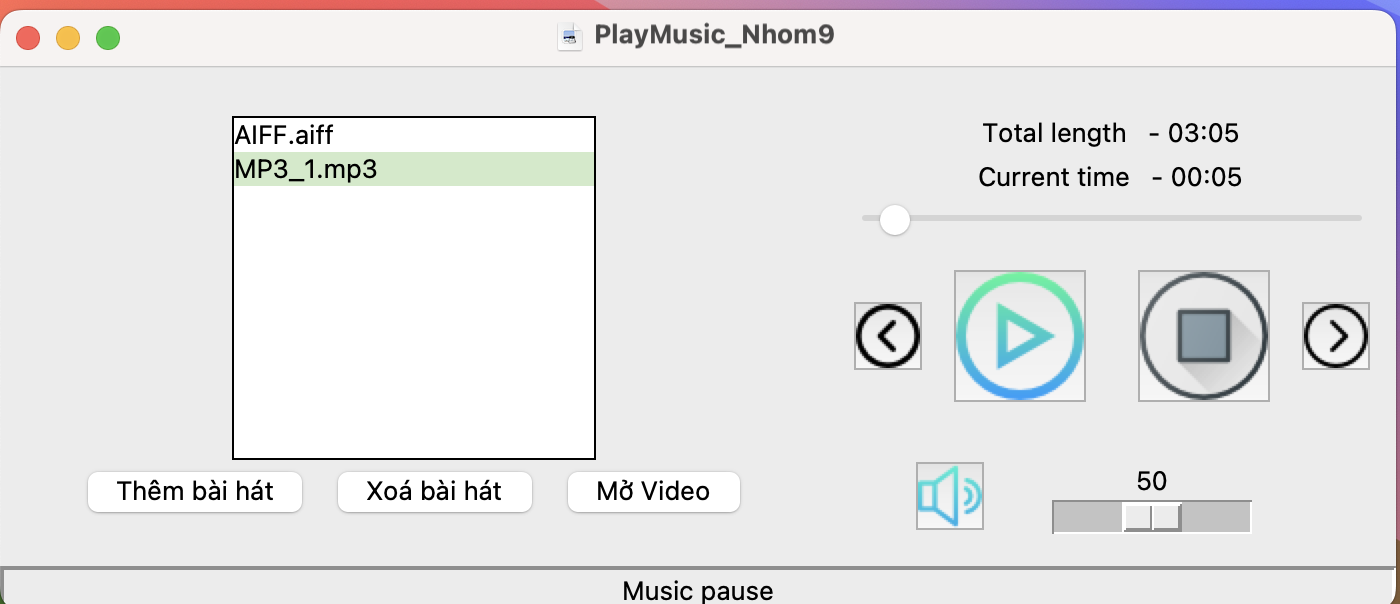
\includegraphics[width=1\linewidth]{template_SGU 2/giaodien.png}
\end{center}
\hspace*{0.5cm} Màn hình chính phần mềm gồm một Lisbox để chứa danh sách bài hát. Kế bên đó là hiển thị chi tiết bài hát như tổng thời gian, thời gian bài hát đang chạy và tên bài hát được thiết lập dưới thanh status. Và đầy đủ các nút chức năng: thanh điều chỉnh thời gian, nút play, nút pause, nút stop, nút previous, nút next, nút add thêm bài hát, nút delete bài hát, nút play video, nút điều chỉnh âm lượng và nút tắt âm lượng.

\noindent --- Giao diện thêm danh sách bài hát:

\hspace  Khi ấn nút thêm bài hát sẽ mở folder để thêm bài hát từ máy tính.
\begin{center}
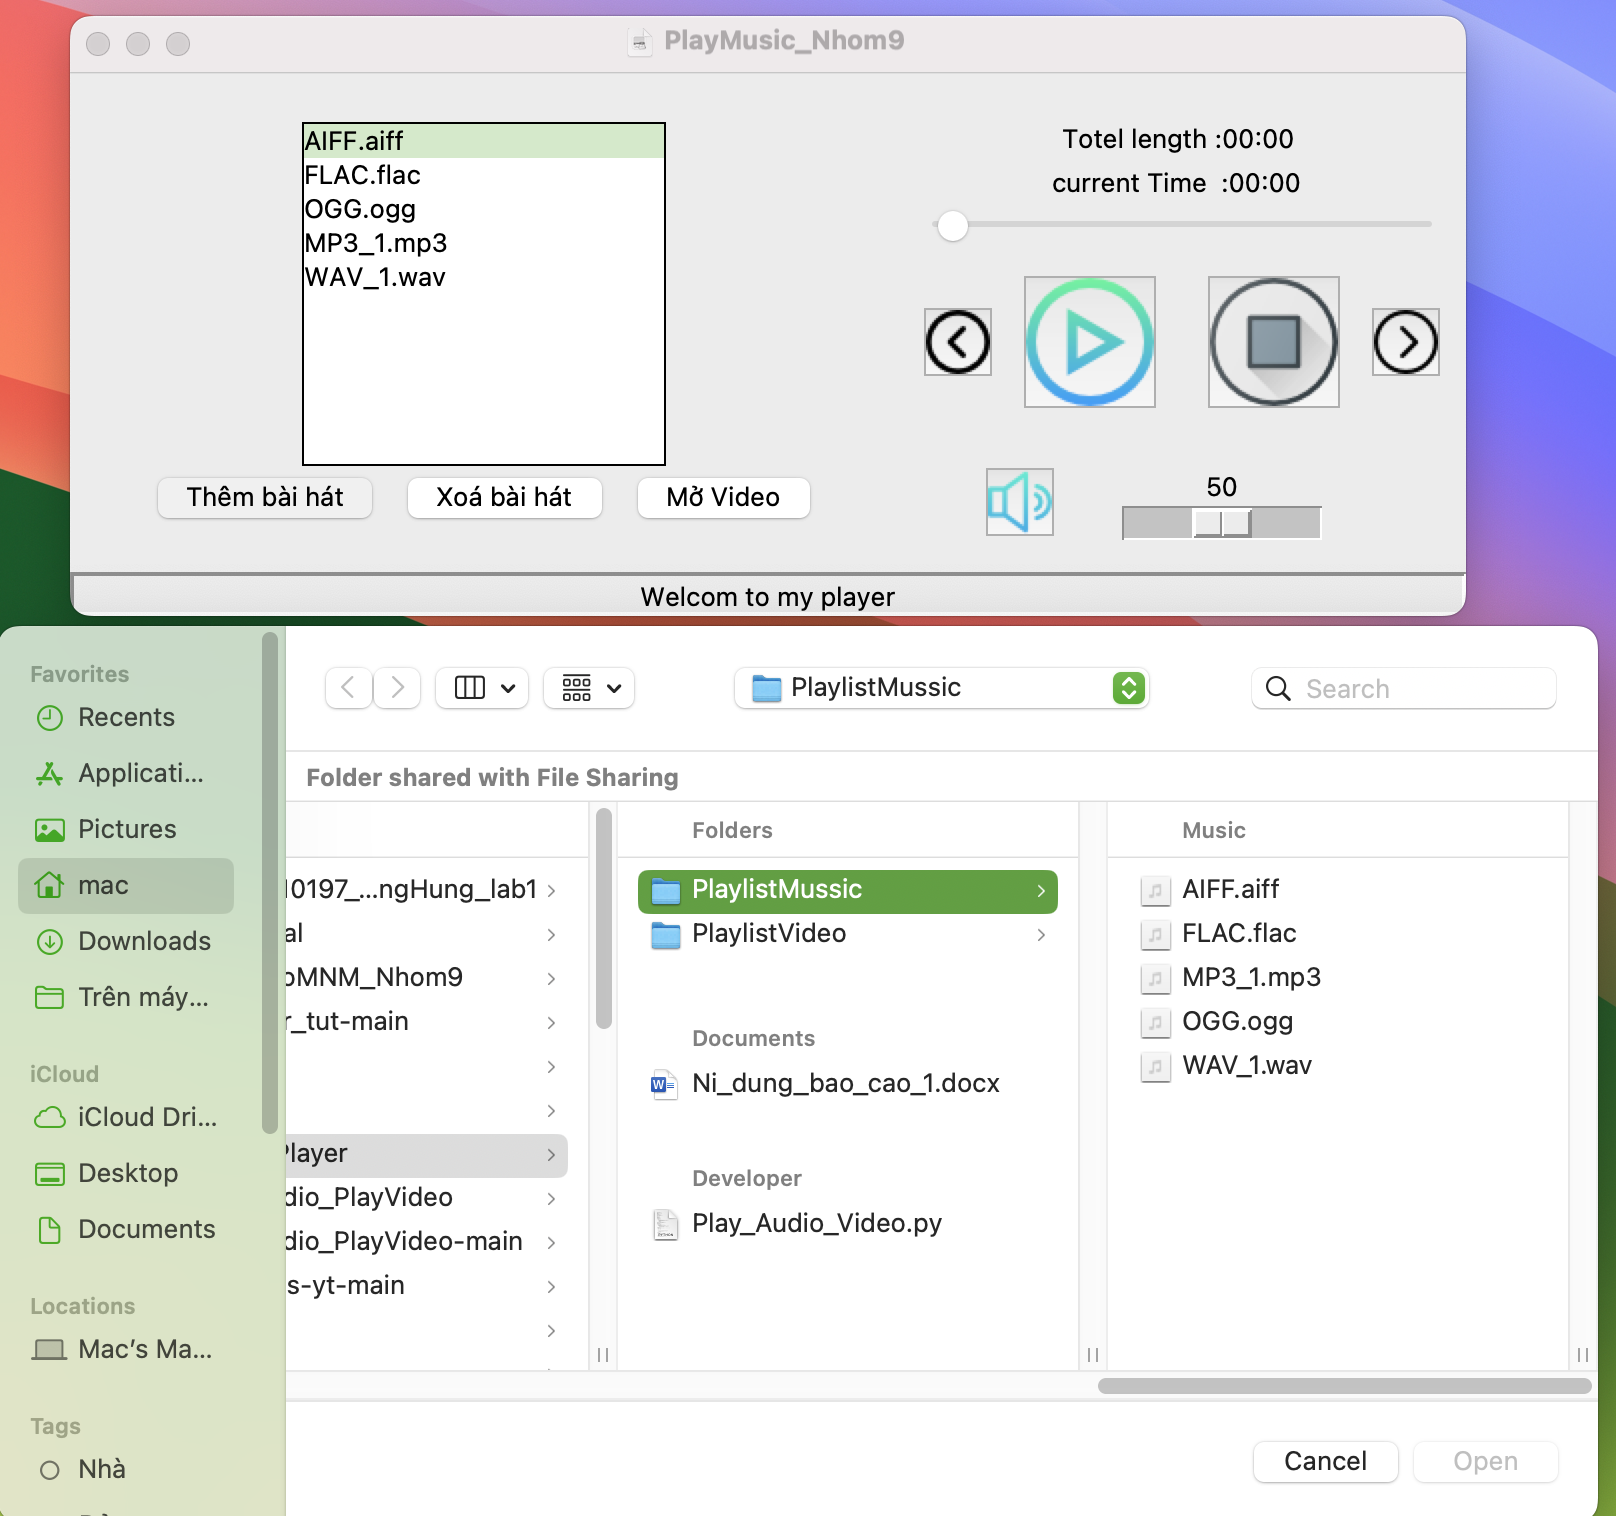
\includegraphics[width=1\linewidth]{template_SGU 2/thembaihat.png}
\end{center} 
\newpage
\hspace  Khi thêm thành công bài hát mới được thêm sẽ được hiển thị ở cuối danh sách được thêm.

\noindent --- Giao diện play video:

\hspace Khi ấn nút mở video thì giao diện sẽ mở fouder của người dùng lên và sau đó người dùng có thể chọn những tệp video mà phần mềm cho phép.
\begin{center}
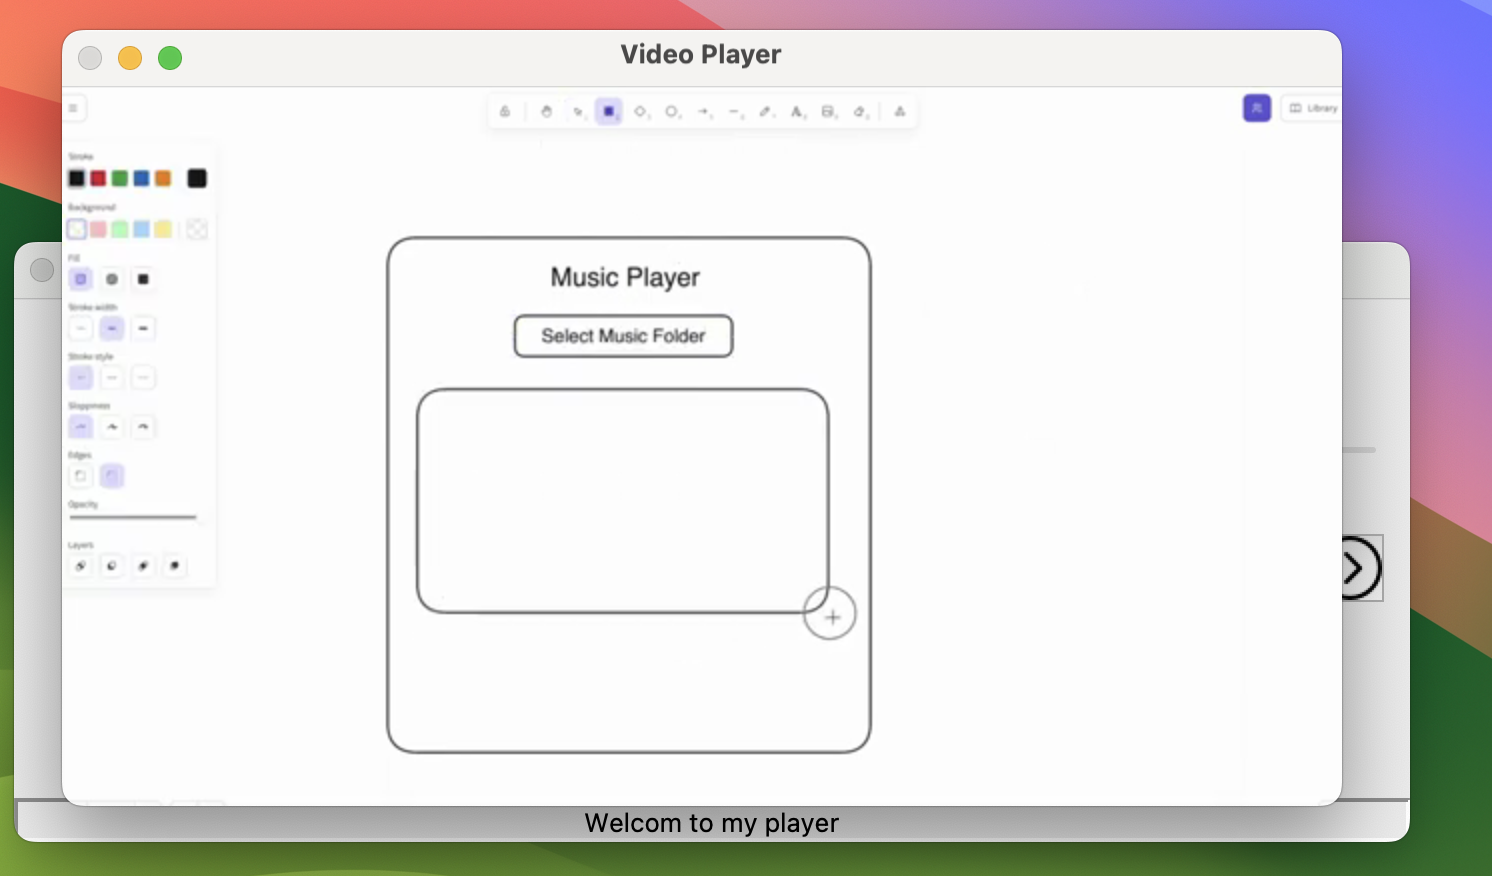
\includegraphics[width=1\linewidth]{template_SGU 2/playvideo.png}
\end{center} 
\hspace  Khi người dùng ấn chọn thì hệ thống sẽ tự động mở video bằng cách gọi thư viện của OpenCV với một fram mới có tên là playVideo. Khi người dùng muốn tắt chúng thì có thể ấn phím "q"
\newpage
\section{Cài đặt vày chạy ứng dụng}
\begin{itemize}
    \item \textbf{Clone project từ git:}     
    \begin{verbatim}
    git clone https://github.com/hung573/PlayAudio\_PlayVideo
    \end{verbatim} 
    \item \textbf{Chuyển tới fouder vừa được clone}     
    \begin{verbatim}
    cd PlayAudio\_PlayVideo
    \end{verbatim} 
    \item \textbf{Run app}     
    \begin{verbatim}
    python main.py
    \end{verbatim}
\end{itemize}
\hspace*{0.5cm}Trước khi chạy ứng dụng, đảm bảo bạn đã cài đặt các phụ thuộc sau:
\begin{itemize}
    \item Python 3.x
    \item Tkinter
    \item Pygame
    \item OS
    \item Mutagen
    \item Time
    \item Threading
    \item OpenCV
\end{itemize}
\subsection{Hướng dẫn cài đặt trên hệ điều hành Windows, Linux, MacOS}
\begin{itemize}
    \item \textbf{Tải Python:} Truy cập trang web chính thức của Python tại \url{https://www.python.org/downloads/} và tải xuống phiên bản Python 3.x phù hợp với hệ điều hành Windows của bạn. Sau đó, chạy tệp cài đặt và tuân theo hướng dẫn trên màn hình để hoàn thành quá trình cài đặt. Hoặc nếu bạn có HomeDrew thì có thể cài đặt Python qua HomeDrew bằng câu lệnh như sau:    
    \begin{verbatim}
    brew install python3
    \end{verbatim} 
     \item \textbf{Kiểm tra:} Sau khi bạn đã cài đặt Python xong thì bạn có thể kiểm tra đã thành công chưa bằng câu lệnh sau:
    \begin{verbatim}
    python3 --version
    \end{verbatim}
    \item \textbf{Cài đặt Pygame, Mutagen, OpenCV:} Mở Command Prompt (cmd) Nếu là MacOS/Linux thì bạn mở Terminal chạy lệnh sau để cài đặt các thư viện:
    \begin{verbatim}
    pip3 install pygame
    pip3 install mutagen
    pip3 install opencv-python-headless
    \end{verbatim}   
\end{itemize}
\hspace*{0.5cm} Sau khi bạn đã cài đặt được tất cả thư viện ở trên thì bạn có thể quay trở lại dùng câu lệnh "python main.py" để bắt đầu run app.

\section{Kết luận}

\hspace Trong quá trình thực hiện dự án phát triển phần mềm mã nguồn mở  PlayerAudio\_PlayderVideo , chúng em đã tích lũy được nhiều kỹ năng và kiến thức mới về lập trình, quản lý dự án và phát triển phần mềm. Mục tiêu của dự án là tạo ra một ứng dụng phát nhạc đơn giản, tiện ích và miễn phí cho người dùng.

\hspace Các điểm mạnh của phần mềm là giao diện người dùng thân thiện và các tính năng phát nhạc cơ bản được hiện thực một cách linh hoạt. Chúng tôi đã xây dựng một giao diện cho phép người dùng thêm, xóa các bài hát vào danh sách phát, cũng như điều khiển các thao tác như phát, tạm dừng, tiếp tục và dừng.

\hspace Tuy nhiên, dự án vẫn còn một số hạn chế và cần được cải thiện trong tương lai như: Chưa có tính năng lập lại bài hát hoặc chọn chế độ random bài hát và cần phát triển thêm về phần chọn danh sách bài hát được yêu thích và tìm kiếm bài hát. Đó là những hạn chế của nhóm em.

\hspace Trong quá trình phát triển phần mềm, chúng em  không thể không bày tỏ lòng biết ơn sâu sắc đến giáo viên hướng dẫn  Từ Lãng Phiêu đã cung cấp cho chúng em sự hỗ trợ và những chỉ dẫn quý báu đã luôn đồng hành và hỗ trợ chúng em đễ chúng em có thể hoàn thành triển khai và phát triển ứng dụng.

\hspace Trong tương lai, chúng em sẽ tục phát triển và nâng cấp phần mềm Audio Player để cải thiện trải nghiệm người dùng và đáp ứng được nhu cầu ngày càng đa dạng của cộng đồng. Chúng em rất mong nhận được sự phản hồi và góp ý từ người dùng và thầy để có thể phát triển sản phẩm tốt hơn. Nhóm chúng em xin chân thành cảm ơn!
\newpage
%%%%%%%%%%%%%%%%%%%%%%%%%%%%%%%%%
\begin{thebibliography}{80}

\bibitem{py la gi}
Python Là Gì? Tất Tần Tật Về Ngôn Ngữ Lập Trình Python:
\href{https://s.net.vn/KIrI}{https://s.net.vn/KIrI}, truy cập ngày 28/4/2024.
\bibitem{py}
Python là gì? Các kiến thức cần biết về lập trình Python:
\href{https://s.net.vn/l8Eq}{https://s.net.vn/l8Eq}, truy cập ngày 28/4/2024.
\bibitem{py_tkinter}
Tkinter Python là gì? Tất cả những gì bạn cần biết về Tkinter:
\href{https://www.icantech.vn/kham-pha/tkinter}{https://www.icantech.vn/kham-pha/tkinter}, truy cập ngày 28/4/2024.
\end{thebibliography}
\end{document}

